% 图 74.2 —— 由 `checks/emit_hand.py` 自动拼出（probe 精测 + prims2 图元分解）
%%
% ⚠ 这是**稿子不是成品**：跑 `checks/checkhand.py 74.2` 看指标 + 看叠合图。
%%
%% ⚠ 待核：
%   · 本图 probe 报出阴影族 1 个 —— **本脚本不生成阴影**（要照原书手写）；prims2 的 strokes 里可能含阴影线，核对时留意别画重
%   · 可疑字形 2 项（空心圈 ⊙ 常被认成字母 o）—— 见文件末
%%
\documentclass[12pt]{standalone}
\usepackage{fontspec}
\setsansfont{Arial}
\newfontfamily\mfallback{DejaVu Sans}
\usepackage{tikz}
\begin{document}
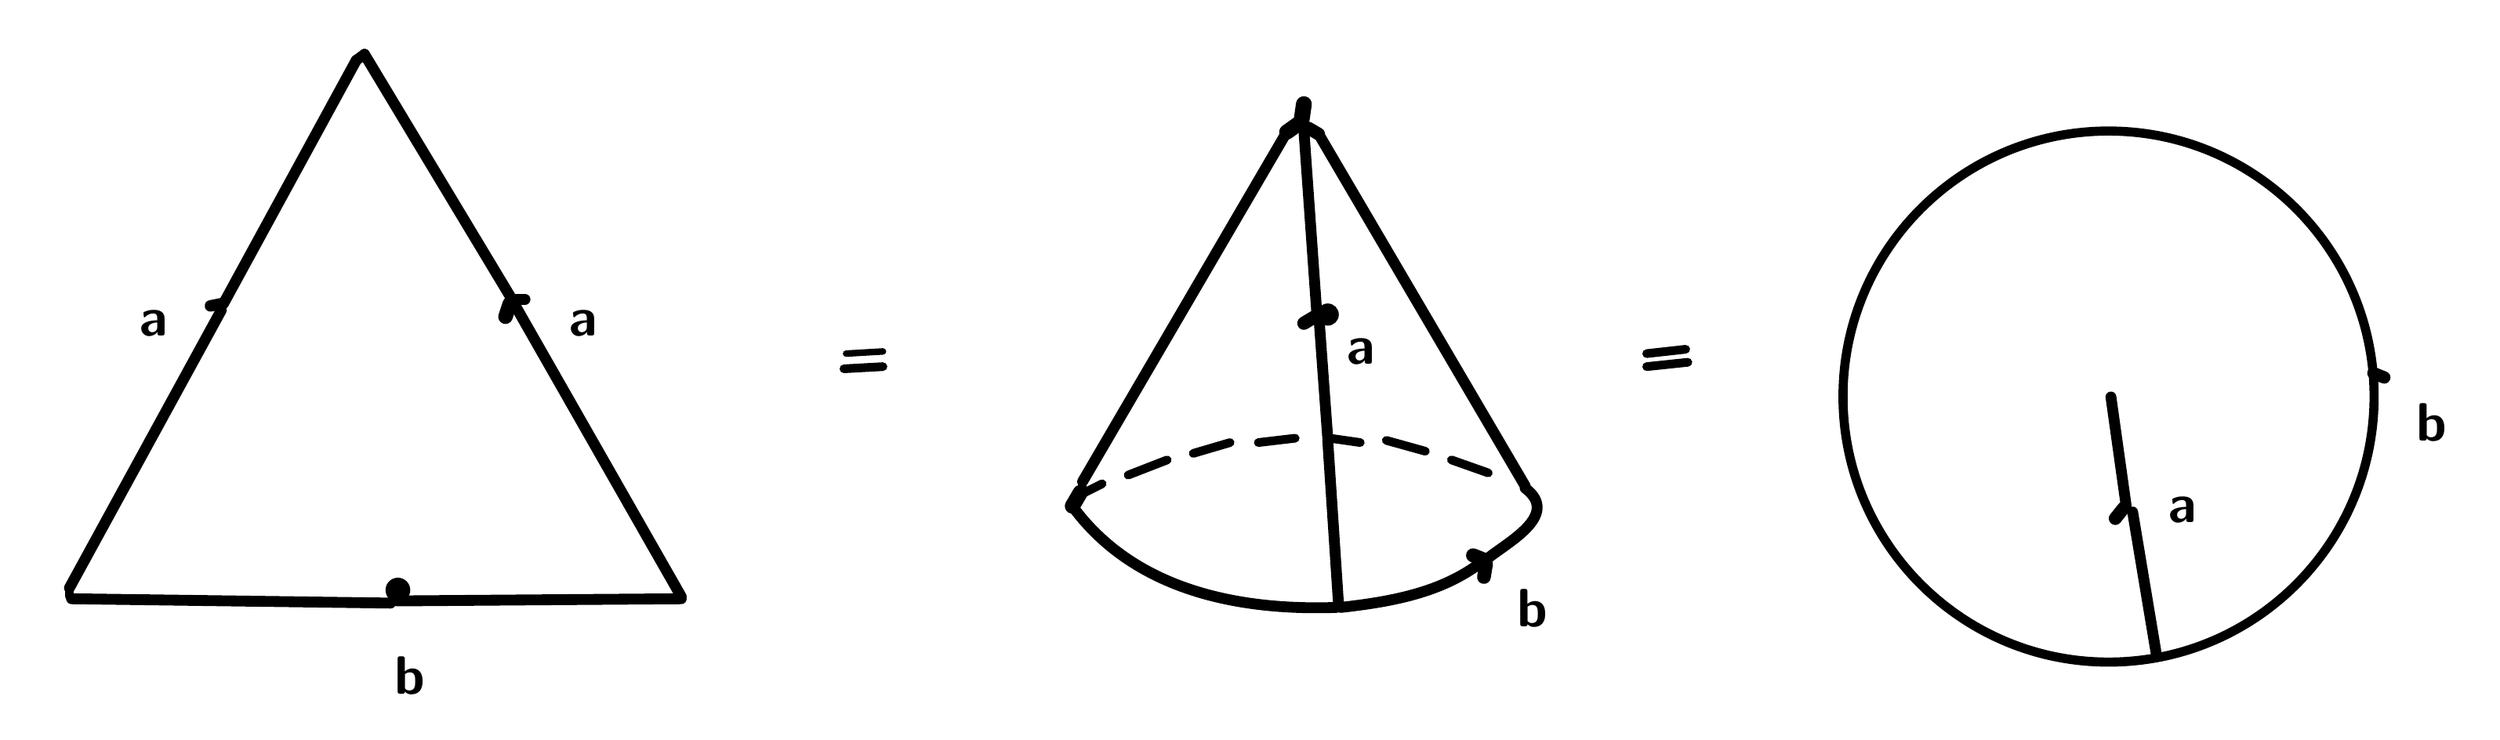
\begin{tikzpicture}[x=1pt, y=-1pt, line width=4.2pt, line cap=round, line join=round]

  %% ════ 填充区（prims2 的 fills）════

  %% ════ 直线段（prims2 的 strokes）════
  \draw[line width=6.7pt] (225.0,130.0) -- (223.0,136.0);
  \draw[line width=4.9pt] (158.0,15.0) -- (154.2,17.8);
  \draw[line width=5.0pt] (154.2,17.8) -- (93.0,130.0);
  \draw[line width=5.0pt] (158.0,15.0) -- (226.0,128.0);
  \draw[line width=4.0pt] (22.0,265.0) -- (22.0,261.0);
  \draw[line width=5.0pt] (22.0,261.0) -- (92.0,133.0);
  \draw[line width=5.0pt] (973.0,226.0) -- (984.0,292.0);
  \draw[line width=5.0pt] (227.0,128.0) -- (232.0,128.0);
  \draw[line width=5.0pt] (602.0,192.0) -- (598.0,137.0);
  \draw[line width=5.0pt] (23.0,266.0) -- (170.0,268.0);
  \draw[line width=5.0pt] (591.0,50.0) -- (597.0,135.0);
  \draw[line width=5.0pt] (227.0,130.0) -- (304.0,265.0);
  \draw[line width=5.0pt] (963.0,173.0) -- (970.0,223.0);
  \draw[line width=5.3pt] (92.0,130.0) -- (87.0,131.0);
  \draw[line width=4.0pt] (676.0,208.0) -- (659.0,202.0);
  \draw[line width=4.0pt] (749.0,153.0) -- (767.0,151.0);
  \draw[line width=6.5pt] (669.0,246.0) -- (674.0,248.0);
  \draw[line width=5.7pt] (1084.0,162.0) -- (1089.0,164.0);
  \draw[line width=7.3pt] (590.0,45.0) -- (591.0,38.0);
  \draw[line width=6.3pt] (675.0,250.0) -- (674.0,256.0);
  \draw[line width=4.0pt] (749.0,159.0) -- (768.0,157.0);
  \draw[line width=5.0pt] (304.0,266.0) -- (173.0,267.0);
  \draw[line width=4.0pt] (540.0,199.0) -- (557.0,194.0);
  \draw[line width=4.0pt] (617.0,194.0) -- (603.0,192.0);
  \draw[line width=6.0pt] (969.0,224.0) -- (965.0,229.0);
  \draw[line width=4.0pt] (397.0,159.0) -- (379.0,160.0);
  \draw[line width=6.1pt] (596.0,136.0) -- (591.0,139.0);
  \draw[line width=5.0pt] (602.0,193.0) -- (607.0,269.0);
  \draw[line width=4.0pt] (510.0,209.0) -- (528.0,202.0);
  \draw[line width=4.0pt] (498.0,213.0) -- (490.0,217.0);
  \draw[line width=7.0pt] (488.0,217.0) -- (484.3,223.3);
  \draw[line width=5.0pt] (693.0,214.0) -- (597.8,51.8);
  \draw[line width=5.9pt] (597.8,51.8) -- (593.0,49.0);
  \draw[line width=3.0pt] (380.0,153.0) -- (397.0,152.0);
  \draw[line width=4.0pt] (629.0,193.0) -- (647.0,198.0);
  \draw[line width=4.0pt] (587.0,192.0) -- (570.0,194.0);
  \draw[line width=4.0pt] (489.0,216.0) -- (489.0,212.0);
  \draw[line width=5.0pt] (489.0,212.0) -- (583.1,50.9);
  \draw[line width=7.0pt] (583.1,50.9) -- (590.0,46.0);

  %% ════ 曲线（prims2 的 curves —— 三段式，坐标同为 (y,x)）════
  \draw[line width=5.0pt] (675.0,248.0) .. controls (684.1,240.3) and (709.7,227.6) .. (693.0,215.0);
  \draw[line width=5.0pt] (484.3,223.3) .. controls (512.4,261.7) and (560.0,271.6) .. (606.0,270.0);
  \draw[line width=5.0pt] (673.0,249.0) .. controls (654.4,263.4) and (630.9,267.4) .. (608.0,270.0);

  %% ════ 圆 / 椭圆（probe 精测）════
  \draw (961.9,172.8) circle (122.4);

  %% ════ 实心点 ════
  \fill (602.0,135.0) circle (5.1);
  \fill (173.4,262.0) circle (5.7);

  %% ════ 标签（probe 直接给的 \node 行）════
  %% ⚠ 全部补了 fill=white：文字在最上层，否则与曲线交叉干扰
     \node[anchor=center,inner sep=0pt,fill=white,font=\fontsize{32.0}{40.0}\selectfont] at (61.1,139.1) {\textsf{\textbf{\textit{a}}}};   % box(52,129,16,17)
     \node[anchor=center,inner sep=0pt,fill=white,font=\fontsize{32.0}{40.0}\selectfont] at (259.1,139.1) {\textsf{\textbf{\textit{a}}}};   % box(250,129,16,17)
     \node[anchor=center,inner sep=0pt,fill=white,font=\fontsize{33.0}{41.2}\selectfont] at (617.6,152.1) {\textsf{\textbf{\textit{a}}}};   % box(608,142,17,17)
     \node[anchor=center,inner sep=0pt,fill=white,font=\fontsize{30.7}{38.3}\selectfont] at (1110.8,184.8) {\textsf{\textbf{\textit{b}}}};   % box(1101,172,17,23)
     \node[anchor=center,inner sep=0pt,fill=white,font=\fontsize{32.0}{40.0}\selectfont] at (996.1,225.1) {\textsf{\textbf{\textit{a}}}};   % box(987,215,16,17)
     \node[anchor=center,inner sep=0pt,fill=white,font=\fontsize{29.1}{36.4}\selectfont] at (696.2,270.2) {\textsf{\textbf{\textit{b}}}};   % box(687,258,16,22)
     \node[anchor=center,inner sep=0pt,fill=white,font=\fontsize{30.0}{37.5}\selectfont] at (178.8,301.2) {\textsf{\textbf{\textit{b}}}};   % box(169,289,17,22)

  % 钉死画布：否则超出的图元/控制点会把页面撑大，1:1 回比就失准
  \pgfresetboundingbox
  \path[use as bounding box] (0,0) rectangle (1132,321);
\end{tikzpicture}
\end{document}

% ⚠ 待核清单（probe 拿不准，人眼过一遍）：
%   · 未识别/跳过：⑤ 跳过/未识别的字形
%   · 未识别/跳过：box(659,201,20,10)
